\chapter{RE-035 Mandatory Layout Envelope And Constraint Negotiation}\label{record-163}

\noindent{\footnotesize\color{BookMuted}\path{docs/design/RE-035-mandatory-layout-envelope-and-constraint-negotiation.md}\par}\smallskip

\begin{RecordMeta}
title: RE-035 Mandatory Layout Envelope And Constraint Negotiation
legend: RE
lane: design

\end{RecordMeta}

\emph{Cycle for making layout envelopes mandatory before any visible UI node can render}

Legend:

\begin{itemize}
\tightlist
\item
  \href{https://github.com/flyingrobots/bijou/blob/1853ad902f6bf219326409e7f743a5a1d6517dbc/docs/legends/RE-runtime-engine.md}{RE - Runtime Engine}
\end{itemize}

Depends on:

\begin{itemize}
\tightlist
\item
  \href{https://github.com/flyingrobots/bijou/blob/cbd70612140e7a450d764b3c7be1c6af878b99bc/docs/design/RE-003-retain-layout-trees-and-layout-invalidation.md}{RE-003}
\item
  \href{https://github.com/flyingrobots/bijou/blob/cbd70612140e7a450d764b3c7be1c6af878b99bc/docs/design/RE-004-route-input-through-layouts-and-layer-bubbling.md}{RE-004}
\item
  \href{https://github.com/flyingrobots/bijou/blob/cbd70612140e7a450d764b3c7be1c6af878b99bc/docs/design/RE-006-formalize-component-layout-and-interaction-contracts.md}{RE-006}
\item
  \href{https://github.com/flyingrobots/bijou/blob/cbd70612140e7a450d764b3c7be1c6af878b99bc/docs/design/DX-022-layout-inspector-overlay.md}{DX-022 - Layout Inspector Overlay}
\item
  \href{https://github.com/flyingrobots/bijou/blob/cbd70612140e7a450d764b3c7be1c6af878b99bc/docs/design/DX-026-mode-lowering-linter.md}{DX-026 - Mode-Lowering Linter}
\end{itemize}

\section{Why This Cycle Exists}\label{record-163-why-this-cycle-exists}

Bijou already has retained runtime seams, layout-driven routing, component metadata, focus maps, inspectors, and mode-lowering tools. The missing floor is that visible UI is still allowed to exist as rendered output before it resolves through a mandatory layout envelope.

That leaves too much behavior implicit:

\begin{itemize}
\tightlist
\item
  components can choose private sizing rules
\item
  renderers can effectively decide geometry while painting
\item
  overflow and clipping have no shared prerequisite contract
\item
  direction-aware placement can drift into physical left/right assumptions
\item
  later workspace features can mutate geometry unless there is a stricter boundary to compile into
\end{itemize}

RE-035 establishes the first boring law: every visible node must resolve a layout envelope before rendering.

\section{North Star}\label{record-163-north-star}

Bijou layout is a retained, semantic, cell-native constraint negotiation system: constraints flow down, preferences flow up, assigned rectangles flow down, and semantic truth lowers outward into interactive, static, pipe, and accessible modes.

The boundary:

\begin{itemize}
\tightlist
\item
  Layout lays out.
\item
  Workspace organizes.
\item
  Interaction commands.
\item
  Renderer paints.
\item
  Modes lower.
\item
  Inspector explains.
\end{itemize}

\section{Human Users / Jobs / Hill}\label{record-163-human-users-jobs-hill}

\subsection{Primary Human Users}\label{record-163-primary-human-users}

\begin{itemize}
\tightlist
\item
  Bijou maintainers turning layout from render-time convention into runtime truth.
\item
  Component authors who need predictable sizing, clipping, and placement rules without copying CSS or Auto Layout.
\item
  DOGFOOD builders who need narrow, standard, and wide documentation layouts to share one inspectable geometry model.
\end{itemize}

\subsection{Human Jobs}\label{record-163-human-jobs}

\begin{enumerate}
\def\labelenumi{\arabic{enumi}.}
\tightlist
\item
  Define a visible node's layout contract before it renders.
\item
  Read min, preferred, max, and assigned size facts without reverse-engineering a renderer.
\item
  Trust parent-owned rectangle assignment instead of child-owned geometry mutation.
\item
  Explain why stack and place containers assigned a particular integer-cell rectangle.
\end{enumerate}

\subsection{Human Hill}\label{record-163-human-hill}

A maintainer can inspect a visible UI node and answer its identity, role, constraints, preferences, assigned rectangle, direction, and assignment reason before looking at the rendered surface.

\section{Agent Users / Jobs / Hill}\label{record-163-agent-users-jobs-hill}

\subsection{Primary Agent Users}\label{record-163-primary-agent-users}

\begin{itemize}
\tightlist
\item
  Agents preparing tests for layout and viewport behavior.
\item
  Agents explaining why a component received a rectangle or could not satisfy a constraint.
\item
  Agents generating future component or workspace code that must compile into primitive layout instead of mutating geometry directly.
\end{itemize}

\subsection{Agent Jobs}\label{record-163-agent-jobs}

\begin{enumerate}
\def\labelenumi{\arabic{enumi}.}
\tightlist
\item
  Read a layout envelope as plain facts.
\item
  Predict whether a child preference can affect parent assignment.
\item
  Generate deterministic assertions for stack assignment, place alignment, and RTL inline-start/inline-end mapping.
\item
  Distinguish surface or buffer cell extents from text-to-cell measurement.
\end{enumerate}

\subsection{Agent Hill}\label{record-163-agent-hill}

An agent can explain a layout decision from mode-neutral facts: incoming constraints, child preferences, parent assignment, integer rounding, direction, and the reason attached to the resolved rectangle.

\section{Concept Diagrams}\label{record-163-concept-diagrams}

These Mermaid diagrams are explanatory mockups, not implementation artifacts. They favor Obsidian-readable semantic structure over raw SVG detail in this cycle doc.

\begin{center}
\BookDiagram{%
\begin{tikzpicture}[booknode/.style={draw=BookHeading,line width=.6pt,fill=BookPanel,rounded corners=1.5pt,align=center,text width=29mm,minimum height=10mm,inner sep=5pt,font=\small},bookedge/.style={-{Latex[length=2mm]},draw=BookHeading,line width=.65pt},every edge quotes/.style={font=\scriptsize,fill=white,inner sep=2pt,text=BookMuted}]
\node[booknode] (Parent) at (0,0) {Parent container / owns assignment};
\node[booknode] (ChildA) at (-3.4,-3.8) {Child A / reports min / preferred / max};
\node[booknode] (ChildB) at (3.4,-3.8) {Child B / reports min / preferred / max};
\node[booknode] (Renderer) at (0,-7.4) {Renderer / paints assigned layout truth};
\draw[bookedge,bend left=12] (Parent) to node[midway,fill=white,inner sep=1.5pt,font=\scriptsize,text=BookMuted] {constraints down} (ChildA);
\draw[bookedge,bend left=32] (Parent) to node[midway,fill=white,inner sep=1.5pt,font=\scriptsize,text=BookMuted] {constraints down} (ChildB);
\draw[bookedge,bend left=52] (ChildA) to node[midway,fill=white,inner sep=1.5pt,font=\scriptsize,text=BookMuted] {preferences up} (Parent);
\draw[bookedge,bend left=12] (ChildB) to node[midway,fill=white,inner sep=1.5pt,font=\scriptsize,text=BookMuted] {preferences up} (Parent);
\draw[bookedge,bend left=32] (Parent) to node[midway,fill=white,inner sep=1.5pt,font=\scriptsize,text=BookMuted] {assigned rects down} (ChildA);
\draw[bookedge,bend left=52] (Parent) to node[midway,fill=white,inner sep=1.5pt,font=\scriptsize,text=BookMuted] {assigned rects down} (ChildB);
\draw[bookedge,bend left=12] (ChildA) to node[midway,fill=white,inner sep=1.5pt,font=\scriptsize,text=BookMuted] {assigned surface region} (Renderer);
\draw[bookedge,bend left=32] (ChildB) to node[midway,fill=white,inner sep=1.5pt,font=\scriptsize,text=BookMuted] {assigned surface region} (Renderer);
\end{tikzpicture}}
\end{center}

Measure/assign protocol: constraints flow down, preferences flow up, assigned rectangles flow down.

\begin{center}
\BookDiagram[.9\linewidth]{%
\begin{tikzpicture}[classbox/.style={draw=BookHeading,fill=BookPanel,line width=.6pt,rounded corners=1.5pt,text width=37mm,align=left,inner sep=5pt,font=\scriptsize},rel/.style={-{Latex[length=2mm]},draw=BookHeading,line width=.6pt}]
\node[classbox] (LayoutEnvelope) at (4.7,0) {\textbf{LayoutEnvelope}\\[-2pt]\rule{\linewidth}{.3pt}\\string id\\string role\\LayoutDirection direction\\LayoutConstraints constraints\\LayoutPreference preference\\AssignedLayoutRect assigned};
\node[classbox] (LayoutConstraints) at (0,-7) {\textbf{LayoutConstraints}\\[-2pt]\rule{\linewidth}{.3pt}\\number minInline\\number | unbounded maxInline\\number minBlock\\number | unbounded maxBlock};
\node[classbox] (LayoutPreference) at (4.7,-7) {\textbf{LayoutPreference}\\[-2pt]\rule{\linewidth}{.3pt}\\number minInline\\number preferredInline\\number | unbounded maxInline\\number minBlock\\number preferredBlock\\number | unbounded maxBlock};
\node[classbox] (AssignedLayoutRect) at (9.4,-7) {\textbf{AssignedLayoutRect}\\[-2pt]\rule{\linewidth}{.3pt}\\number inlineStart\\number blockStart\\number inlineSize\\number blockSize};
\draw[rel,{Diamond[length=2mm]}-] (LayoutEnvelope) to node[midway,fill=white,inner sep=2pt,font=\scriptsize,text=BookMuted,align=center] {} (LayoutConstraints);
\draw[rel,{Diamond[length=2mm]}-] (LayoutEnvelope) to node[midway,fill=white,inner sep=2pt,font=\scriptsize,text=BookMuted,align=center] {} (LayoutPreference);
\draw[rel,{Diamond[length=2mm]}-] (LayoutEnvelope) to node[midway,fill=white,inner sep=2pt,font=\scriptsize,text=BookMuted,align=center] {} (AssignedLayoutRect);
\end{tikzpicture}}
\par\smallskip{\small\color{BookMuted}Explicit layout facts}
\end{center}

A visible node owns explicit layout facts before rendering.

\begin{center}
\BookDiagram{%
\begin{tikzpicture}[booknode/.style={draw=BookHeading,line width=.6pt,fill=BookPanel,rounded corners=1.5pt,align=center,text width=29mm,minimum height=10mm,inner sep=5pt,font=\small},bookedge/.style={-{Latex[length=2mm]},draw=BookHeading,line width=.65pt},every edge quotes/.style={font=\scriptsize,fill=white,inner sep=2pt,text=BookMuted}]
\node[booknode] (V) at (0,0) {Visible Node};
\node[booknode] (E) at (0,-1.7) {Layout Envelope};
\node[booknode] (C) at (-5,-3.6) {Constraints};
\node[booknode] (P) at (-1.7,-3.6) {Preference};
\node[booknode] (A) at (1.7,-3.6) {Assigned Rect};
\node[booknode] (M) at (5,-3.6) {Measured Content Extent};
\node[booknode] (S) at (5,-5.6) {Surface-backed content / reports width / height cells};
\node[booknode] (B) at (5,-7.6) {Buffer-backed content / reports cell extent};
\node[booknode] (T) at (1.7,-5.6) {Text content};
\node[booknode] (TA) at (1.7,-7.6) {Text Measurement Adapter};
\node[booknode] (CE) at (-1.7,-7.6) {Cell Extent};
\node[booknode] (R) at (-1.7,-5.6) {Renderer / paints assigned layout truth};
\draw[bookedge,] (V) to (E);
\draw[bookedge,] (E) to (C);
\draw[bookedge,] (E) to (P);
\draw[bookedge,] (E) to (A);
\draw[bookedge,] (E) to (M);
\draw[bookedge,] (M) to (S);
\draw[bookedge,] (M) to (B);
\draw[bookedge,] (M) to (T);
\draw[bookedge,] (T) to (TA);
\draw[bookedge,] (TA) to (CE);
\draw[bookedge,] (CE) to (P);
\draw[bookedge,] (A) to (R);
\end{tikzpicture}}
\end{center}

Layout measures cell extents. Text measurement is one adapter into the measurement seam, not the canonical layout model.

\begin{CodeBlock}
96 inline cells

[ nav: fixed 24 ][gap 1][ content: flex 52 ][gap 1][ inspector: fixed 18 ]
\end{CodeBlock}

Stack assignment proves the first slice without implementing full flexbox: \texttt{9\allowbreak{}6\allowbreak{} \allowbreak{}a\allowbreak{}v\allowbreak{}a\allowbreak{}i\allowbreak{}l\allowbreak{}a\allowbreak{}b\allowbreak{}l\allowbreak{}e\allowbreak{} \allowbreak{}-\allowbreak{} \allowbreak{}2\allowbreak{}4\allowbreak{} \allowbreak{}n\allowbreak{}a\allowbreak{}v\allowbreak{} \allowbreak{}-\allowbreak{} \allowbreak{}1\allowbreak{}8\allowbreak{} \allowbreak{}i\allowbreak{}n\allowbreak{}s\allowbreak{}p\allowbreak{}e\allowbreak{}c\allowbreak{}t\allowbreak{}o\allowbreak{}r\allowbreak{} \allowbreak{}-\allowbreak{} \allowbreak{}2\allowbreak{} \allowbreak{}g\allowbreak{}a\allowbreak{}p\allowbreak{}s\allowbreak{} \allowbreak{}=\allowbreak{} \allowbreak{}5\allowbreak{}2\allowbreak{} \allowbreak{}f\allowbreak{}l\allowbreak{}e\allowbreak{}x\allowbreak{}i\allowbreak{}b\allowbreak{}l\allowbreak{}e\allowbreak{} \allowbreak{}c\allowbreak{}e\allowbreak{}l\allowbreak{}l\allowbreak{}s}.

\begin{center}
\BookDiagram{%
\begin{tikzpicture}[booknode/.style={draw=BookHeading,line width=.6pt,fill=BookPanel,rounded corners=1.5pt,align=center,text width=29mm,minimum height=10mm,inner sep=5pt,font=\small},bookedge/.style={-{Latex[length=2mm]},draw=BookHeading,line width=.65pt},every edge quotes/.style={font=\scriptsize,fill=white,inner sep=2pt,text=BookMuted}]
\node[booknode] (LTR) at (-4,-2.6) {LTR / inline-start = physical left / inline-end = physical right};
\node[booknode] (RTL) at (0,-2.6) {RTL / inline-start = physical right / inline-end = physical left};
\node[booknode] (Block) at (4,-2.6) {block-start remains physical top / for RE-035 horizontal writing mode};
\node[booknode] (Contract) at (0,0) {Component contract / uses logical start/end};
\draw[bookedge,] (Contract) to (LTR);
\draw[bookedge,] (Contract) to (RTL);
\draw[bookedge,] (Contract) to (Block);
\end{tikzpicture}}
\end{center}

Logical axes let placement flip under RTL without changing source order; the engine derives physical placement from direction.

\section{Human Playback}\label{record-163-human-playback}

\begin{enumerate}
\def\labelenumi{\arabic{enumi}.}
\tightlist
\item
  A DOGFOOD shell renders a header, navigation pane, content pane, and status line.
\item
  The root layout receives a 96-column by 24-row terminal constraint.
\item
  The header and status line report fixed block preferences.
\item
  The navigation pane reports a fixed 24-cell inline preference.
\item
  The content pane reports a flexible inline preference with a useful minimum.
\item
  The parent stack assigns concrete integer rectangles to each child.
\item
  The renderer receives those assigned rectangles and paints clipped surfaces inside them.
\item
  The maintainer opens the layout facts and sees the constraints, preferences, assignment, and reason for the content pane's 52-cell inline span.
\end{enumerate}

\section{Agent Playback}\label{record-163-agent-playback}

\begin{enumerate}
\def\labelenumi{\arabic{enumi}.}
\tightlist
\item
  An agent reads a resolved layout envelope for \texttt{d\allowbreak{}o\allowbreak{}c\allowbreak{}s\allowbreak{}.\allowbreak{}c\allowbreak{}o\allowbreak{}n\allowbreak{}t\allowbreak{}e\allowbreak{}n\allowbreak{}t}.
\item
  It sees the node id, role, direction, incoming constraints, min/preferred/max preferences, assigned rectangle, and assignment reason.
\item
  It verifies that \texttt{d\allowbreak{}o\allowbreak{}c\allowbreak{}s\allowbreak{}.\allowbreak{}c\allowbreak{}o\allowbreak{}n\allowbreak{}t\allowbreak{}e\allowbreak{}n\allowbreak{}t} did not force parent geometry after assignment.
\item
  It verifies that RTL direction maps inline-start to the physical right edge for placement tests.
\item
  It emits a deterministic assertion against the layout facts without parsing rendered text or ANSI output.
\end{enumerate}

\section{Accessibility / Assistive Posture}\label{record-163-accessibility-assistive-posture}

RE-035 does not build the full accessible layout mode. It must still preserve the facts that later accessible output needs:

\begin{itemize}
\tightlist
\item
  stable node identity
\item
  role
\item
  source order
\item
  direction
\item
  assigned rectangle
\item
  mode-neutral reason text
\end{itemize}

The first implementation should not hide semantic identity inside surfaces. Accessible and static output can later lower from the same layout truth rather than trying to recover structure from painted cells.

\section{Localization / Directionality Posture}\label{record-163-localization-directionality-posture}

RE-035 introduces logical axes before any new stack or place behavior can settle into physical left/right assumptions.

The first direction scope is intentionally narrow:

\begin{itemize}
\tightlist
\item
  \texttt{l\allowbreak{}t\allowbreak{}r}
\item
  \texttt{r\allowbreak{}t\allowbreak{}l}
\item
  \texttt{a\allowbreak{}u\allowbreak{}t\allowbreak{}o} as a declared direction value
\item
  horizontal writing mode only
\item
  inline-start and inline-end mapped through direction
\item
  block-start and block-end kept physical top/bottom for this cycle
\end{itemize}

Full bidi text layout, cursor maps, and vertical writing modes belong to later text and localization cycles.

\section{Agent Inspectability / Explainability Posture}\label{record-163-agent-inspectability-explainability-posture}

Every resolved layout node should be explainable as data. The explanation does not need to be a stable public API in the first slice, but tests should prove that the engine can report:

\begin{itemize}
\tightlist
\item
  node id
\item
  role
\item
  direction
\item
  incoming constraints
\item
  min/preferred/max preference facts
\item
  assigned rectangle
\item
  assignment reason
\end{itemize}

The explanation must not require executing renderer behavior or parsing a surface string.

\section{Linked Invariants}\label{record-163-linked-invariants}

\begin{itemize}
\tightlist
\item
  \href{https://github.com/flyingrobots/bijou/blob/cbd70612140e7a450d764b3c7be1c6af878b99bc/docs/invariants/runtime-truth-wins.md}{Runtime Truth Wins}
\item
  \href{https://github.com/flyingrobots/bijou/blob/cbd70612140e7a450d764b3c7be1c6af878b99bc/docs/invariants/layout-owns-interaction-geometry.md}{Layout Owns Interaction Geometry}
\item
  \href{https://github.com/flyingrobots/bijou/blob/cbd70612140e7a450d764b3c7be1c6af878b99bc/docs/invariants/buffer-holds-facts.md}{The Buffer Holds Facts}
\item
  \href{https://github.com/flyingrobots/bijou/blob/cbd70612140e7a450d764b3c7be1c6af878b99bc/docs/invariants/focus-owns-input.md}{Focus Owns Input}
\item
  \href{https://github.com/flyingrobots/bijou/blob/cbd70612140e7a450d764b3c7be1c6af878b99bc/docs/invariants/tests-are-the-spec.md}{Tests Are the Spec}
\end{itemize}

\section{Requirements}\label{record-163-requirements}

\begin{itemize}
\tightlist
\item
  Introduce a pure layout envelope model for visible UI nodes.
\item
  Represent logical axes:

  \begin{itemize}
  \tightlist
  \item
    \texttt{i\allowbreak{}n\allowbreak{}l\allowbreak{}i\allowbreak{}n\allowbreak{}e\allowbreak{}-\allowbreak{}s\allowbreak{}t\allowbreak{}a\allowbreak{}r\allowbreak{}t}
  \item
    \texttt{i\allowbreak{}n\allowbreak{}l\allowbreak{}i\allowbreak{}n\allowbreak{}e\allowbreak{}-\allowbreak{}e\allowbreak{}n\allowbreak{}d}
  \item
    \texttt{b\allowbreak{}l\allowbreak{}o\allowbreak{}c\allowbreak{}k\allowbreak{}-\allowbreak{}s\allowbreak{}t\allowbreak{}a\allowbreak{}r\allowbreak{}t}
  \item
    \texttt{b\allowbreak{}l\allowbreak{}o\allowbreak{}c\allowbreak{}k\allowbreak{}-\allowbreak{}e\allowbreak{}n\allowbreak{}d}
  \end{itemize}
\item
  Represent layout direction at least as \texttt{l\allowbreak{}t\allowbreak{}r}, \texttt{r\allowbreak{}t\allowbreak{}l}, and \texttt{a\allowbreak{}u\allowbreak{}t\allowbreak{}o}.
\item
  Represent size facts separately:

  \begin{itemize}
  \tightlist
  \item
    minimum size
  \item
    preferred size
  \item
    maximum size
  \item
    assigned size
  \end{itemize}
\item
  Represent incoming constraints as bounded, exact, or unbounded per axis.
\item
  Keep parent assignment authoritative.
\item
  Add a deterministic rounding policy for flexible integer-cell tracks.
\item
  Add initial layout containers only where needed to prove the protocol:

  \begin{itemize}
  \tightlist
  \item
    stack
  \item
    place
  \end{itemize}
\item
  Add layout explanation facts suitable for inspectors, tests, and agent output.
\item
  Define the content measurement seam for cell extents. Text measurement is one adapter into that seam, not the canonical layout model.
\item
  Reserve the concept of fit policy so later compression, truncation, wrapping, clipping, and overflow work has a deterministic place to attach.
\end{itemize}

\section{Non-Goals}\label{record-163-non-goals}

\begin{itemize}
\tightlist
\item
  Do not implement full text wrapping, grapheme segmentation, bidi layout, or cursor maps. RE-035 defines the text-to-cell measurement seam; RE-036 owns the text measurement work.
\item
  Do not implement scrollbars, scroll anchoring, virtualized viewports, or marquee behavior.
\item
  Do not implement the full fit-policy/compression ladder. RE-035 names the concept; later responsive, viewport, and text cycles define behavior.
\item
  Do not implement docking, tab dragging, drawers, floating panels, workspace persistence, or drag-and-drop rearrangement.
\item
  Do not introduce a new \texttt{L\allowbreak{}K} legend yet. This is runtime-engine work until the layout kernel becomes its own public subsystem, package, or doctrine track.
\item
  Do not build CSS, Auto Layout, or a general constraint solver.
\end{itemize}

\section{Contract Sketch}\label{record-163-contract-sketch}

The first public or internal names can change during implementation, but the conceptual shape should stay small:

\begin{CodeBlock}
type LayoutDirection = 'ltr' | 'rtl' | 'auto';

type LogicalAxis = 'inline' | 'block';

type LogicalAlign = 'start' | 'center' | 'end' | 'stretch';

type LayoutFitPolicy =
  | 'fixed'
  | 'shrink'
  | 'grow'
  | 'truncate'
  | 'wrap'
  | 'overflow'
  | 'clip'
  | 'priority';

interface LayoutConstraints {
  readonly minInline: number;
  readonly maxInline: number | 'unbounded';
  readonly minBlock: number;
  readonly maxBlock: number | 'unbounded';
}

interface LayoutPreference {
  readonly minInline: number;
  readonly preferredInline: number;
  readonly maxInline: number | 'unbounded';
  readonly minBlock: number;
  readonly preferredBlock: number;
  readonly maxBlock: number | 'unbounded';
}

interface AssignedLayoutRect {
  readonly inlineStart: number;
  readonly blockStart: number;
  readonly inlineSize: number;
  readonly blockSize: number;
}

interface LayoutEnvelope {
  readonly id: string;
  readonly role: string;
  readonly direction: LayoutDirection;
  readonly constraints: LayoutConstraints;
  readonly preference: LayoutPreference;
  readonly assigned: AssignedLayoutRect;
  readonly fit?: LayoutFitPolicy;
}
\end{CodeBlock}

The key rule is not the exact type names. The key rule is that a visible node has explicit constraint, preference, assignment, identity, role, and direction facts before rendering.

\section{Measure And Assign}\label{record-163-measure-and-assign}

RE-035 uses a bounded two-step protocol:

\begin{enumerate}
\def\labelenumi{\arabic{enumi}.}
\tightlist
\item
  Measure: a parent asks children for preferences under incoming constraints.
\item
  Assign: the parent chooses concrete integer rectangles and gives them back to children.
\end{enumerate}

Children may report preferences. They may not force parent size after assignment.

Rendering happens only after assignment.

\section{Layout Fit Policy}\label{record-163-layout-fit-policy}

RE-035 should reserve fit policy as the node's declared posture under compression, expansion, and overflow.

Constraints say what space is possible. Preferences say what size a node wants. Assignment says what rectangle the parent chose. Fit policy says how the node intends to remain useful when those facts disagree.

Examples:

\begin{itemize}
\tightlist
\item
  \texttt{f\allowbreak{}i\allowbreak{}x\allowbreak{}e\allowbreak{}d}: preserve assigned size and let the parent resolve surrounding space
\item
  \texttt{s\allowbreak{}h\allowbreak{}r\allowbreak{}i\allowbreak{}n\allowbreak{}k}: accept less than preferred size before siblings with higher priority
\item
  \texttt{g\allowbreak{}r\allowbreak{}o\allowbreak{}w}: accept extra space after fixed and preferred claims are satisfied
\item
  \texttt{t\allowbreak{}r\allowbreak{}u\allowbreak{}n\allowbreak{}c\allowbreak{}a\allowbreak{}t\allowbreak{}e}: preserve one-line or bounded content by shortening presentation
\item
  \texttt{w\allowbreak{}r\allowbreak{}a\allowbreak{}p}: trade inline space for block space through a measurement adapter
\item
  \texttt{o\allowbreak{}v\allowbreak{}e\allowbreak{}r\allowbreak{}f\allowbreak{}l\allowbreak{}o\allowbreak{}w}: report content extent beyond the assigned rect
\item
  \texttt{c\allowbreak{}l\allowbreak{}i\allowbreak{}p}: hide paint outside the assigned rect without claiming scroll state
\item
  \texttt{p\allowbreak{}r\allowbreak{}i\allowbreak{}o\allowbreak{}r\allowbreak{}i\allowbreak{}t\allowbreak{}y}: participate in an ordered compression ladder
\end{itemize}

The first implementation does not need to execute all of these policies. It should only leave an explicit home for this intent so later text, viewport, responsive, and workspace cycles do not invent private compression rules.

\section{Initial Containers}\label{record-163-initial-containers}

\subsection{Stack}\label{record-163-stack}

\texttt{s\allowbreak{}t\allowbreak{}a\allowbreak{}c\allowbreak{}k} proves ordered layout along one logical axis.

It should support:

\begin{itemize}
\tightlist
\item
  fixed tracks
\item
  flexible tracks
\item
  gaps
\item
  logical direction
\item
  deterministic leftover-cell rounding
\item
  child explanations
\end{itemize}

The first slice does not need full flexbox.

\subsection{Place}\label{record-163-place}

\texttt{p\allowbreak{}l\allowbreak{}a\allowbreak{}c\allowbreak{}e} proves alignment inside an assigned rectangle.

It should support:

\begin{itemize}
\tightlist
\item
  inline alignment: start, center, end, stretch
\item
  block alignment: start, center, end, stretch
\item
  logical start/end resolution under LTR and RTL
\end{itemize}

The first slice does not need absolute positioning, anchors, portals, or overlay placement.

\section{Content Measurement Seam}\label{record-163-content-measurement-seam}

RE-035 layout measures cell extents, not JavaScript string length.

Bijou surfaces are already rectangular grids of cells with \texttt{w\allowbreak{}i\allowbreak{}d\allowbreak{}t\allowbreak{}h} and \texttt{h\allowbreak{}e\allowbreak{}i\allowbreak{}g\allowbreak{}h\allowbreak{}t}. A surface-backed component can report those dimensions directly as its content extent. Text is different only because it must first be lowered into cells through a measurement adapter.

RE-035 should define where content measurement plugs in, but should not solve the whole text system.

The seam should make room for surface and buffer content that can already report:

\begin{itemize}
\tightlist
\item
  inline cell extent
\item
  block cell extent
\item
  optional baseline facts
\item
  optional semantic facts
\end{itemize}

The text adapter into that seam should make room for:

\begin{itemize}
\tightlist
\item
  available inline size
\item
  wrap policy
\item
  overflow policy
\item
  layout direction
\item
  ambiguous-width policy
\item
  output mode
\end{itemize}

The implementation may use a minimal deterministic placeholder for early component tests, but the design must make it clear that no text-bearing component should own private \texttt{t\allowbreak{}e\allowbreak{}x\allowbreak{}t\allowbreak{}.\allowbreak{}l\allowbreak{}e\allowbreak{}n\allowbreak{}g\allowbreak{}t\allowbreak{}h} measurement in the long run. String-to-surface conversion belongs behind the text measurement adapter.

\section{Mode-Neutral Facts}\label{record-163-mode-neutral-facts}

The resolved layout should be inspectable without depending on a rendered surface.

Example facts:

\begin{CodeBlock}
node docs.content
role viewport
direction ltr
constraints inline 0..96 block 0..24
preference inline min 32 preferred 72 max unbounded
preference block min 6 preferred 18 max unbounded
assigned inline-start 24 block-start 1 inline-size 72 block-size 22
reason took remaining inline space in stack after fixed nav and status chrome
\end{CodeBlock}

Interactive, static, pipe, and accessible modes may present these facts differently, but the underlying layout truth should be shared.

\section{Implementation Outline}\label{record-163-implementation-outline}

\begin{enumerate}
\def\labelenumi{\arabic{enumi}.}
\tightlist
\item
  Add a pure layout module that can construct and resolve layout envelopes without rendering.
\item
  Add constraint, preference, assigned-rect, direction, and explanation fact types.
\item
  Add the two-step measure/assign protocol with parent-owned assignment.
\item
  Add minimal stack and place helpers to prove the protocol.
\item
  Add deterministic integer rounding for flexible tracks.
\item
  Add a content measurement seam that accepts surface/buffer cell extents directly and leaves text-to-cell measurement behind an adapter.
\item
  Add a render-facing seam that receives assigned rectangles instead of deriving geometry from rendered output.
\item
  Keep the implementation pure and shell-agnostic.
\end{enumerate}

\section{Design Thinking Slice Plan}\label{record-163-design-thinking-slice-plan}

This cycle uses the Method loop with a Design Thinking posture: sponsored users, measurable Hills, explicit assumptions, low-ceremony prototypes, and playback after each slice. The team should keep asking whether the slice helps a maintainer or agent inspect layout truth before render.

\subsection{Sponsored Users}\label{record-163-sponsored-users}

\begin{itemize}
\tightlist
\item
  Sponsored Human: Bijou maintainer closing the v6 release boundary and auditing layout behavior without parsing painted terminal rows.
\item
  Sponsored Agent: Implementation or review agent generating deterministic assertions against layout facts, not renderer strings.
\end{itemize}

\subsection{Hill For The First Ten Slices}\label{record-163-hill-for-the-first-ten-slices}

A maintainer or agent can construct visible layout nodes, resolve parent-owned integer rectangles through stack and place, inspect the explanation facts, and hand the assigned rectangle to a renderer-facing seam without executing a renderer.

\subsection{Assumptions To Test}\label{record-163-assumptions-to-test}

\begin{itemize}
\tightlist
\item
  A small pure module in \texttt{@\allowbreak{}f\allowbreak{}l\allowbreak{}y\allowbreak{}i\allowbreak{}n\allowbreak{}g\allowbreak{}r\allowbreak{}o\allowbreak{}b\allowbreak{}o\allowbreak{}t\allowbreak{}s\allowbreak{}/\allowbreak{}b\allowbreak{}i\allowbreak{}j\allowbreak{}o\allowbreak{}u} can establish layout truth before DOGFOOD or \texttt{b\allowbreak{}i\allowbreak{}j\allowbreak{}o\allowbreak{}u\allowbreak{}-\allowbreak{}t\allowbreak{}u\allowbreak{}i} adopts it.
\item
  Mandatory render-facing envelopes can be proven as an adapter seam before every existing component is migrated.
\item
  Surface and buffer extents are already cell-native enough to seed the measurement seam.
\item
  Text measurement can remain an adapter placeholder in RE-035 without smuggling JavaScript string length into the canonical layout model.
\end{itemize}

\subsection{Ten Slices}\label{record-163-ten-slices}

\begin{center}
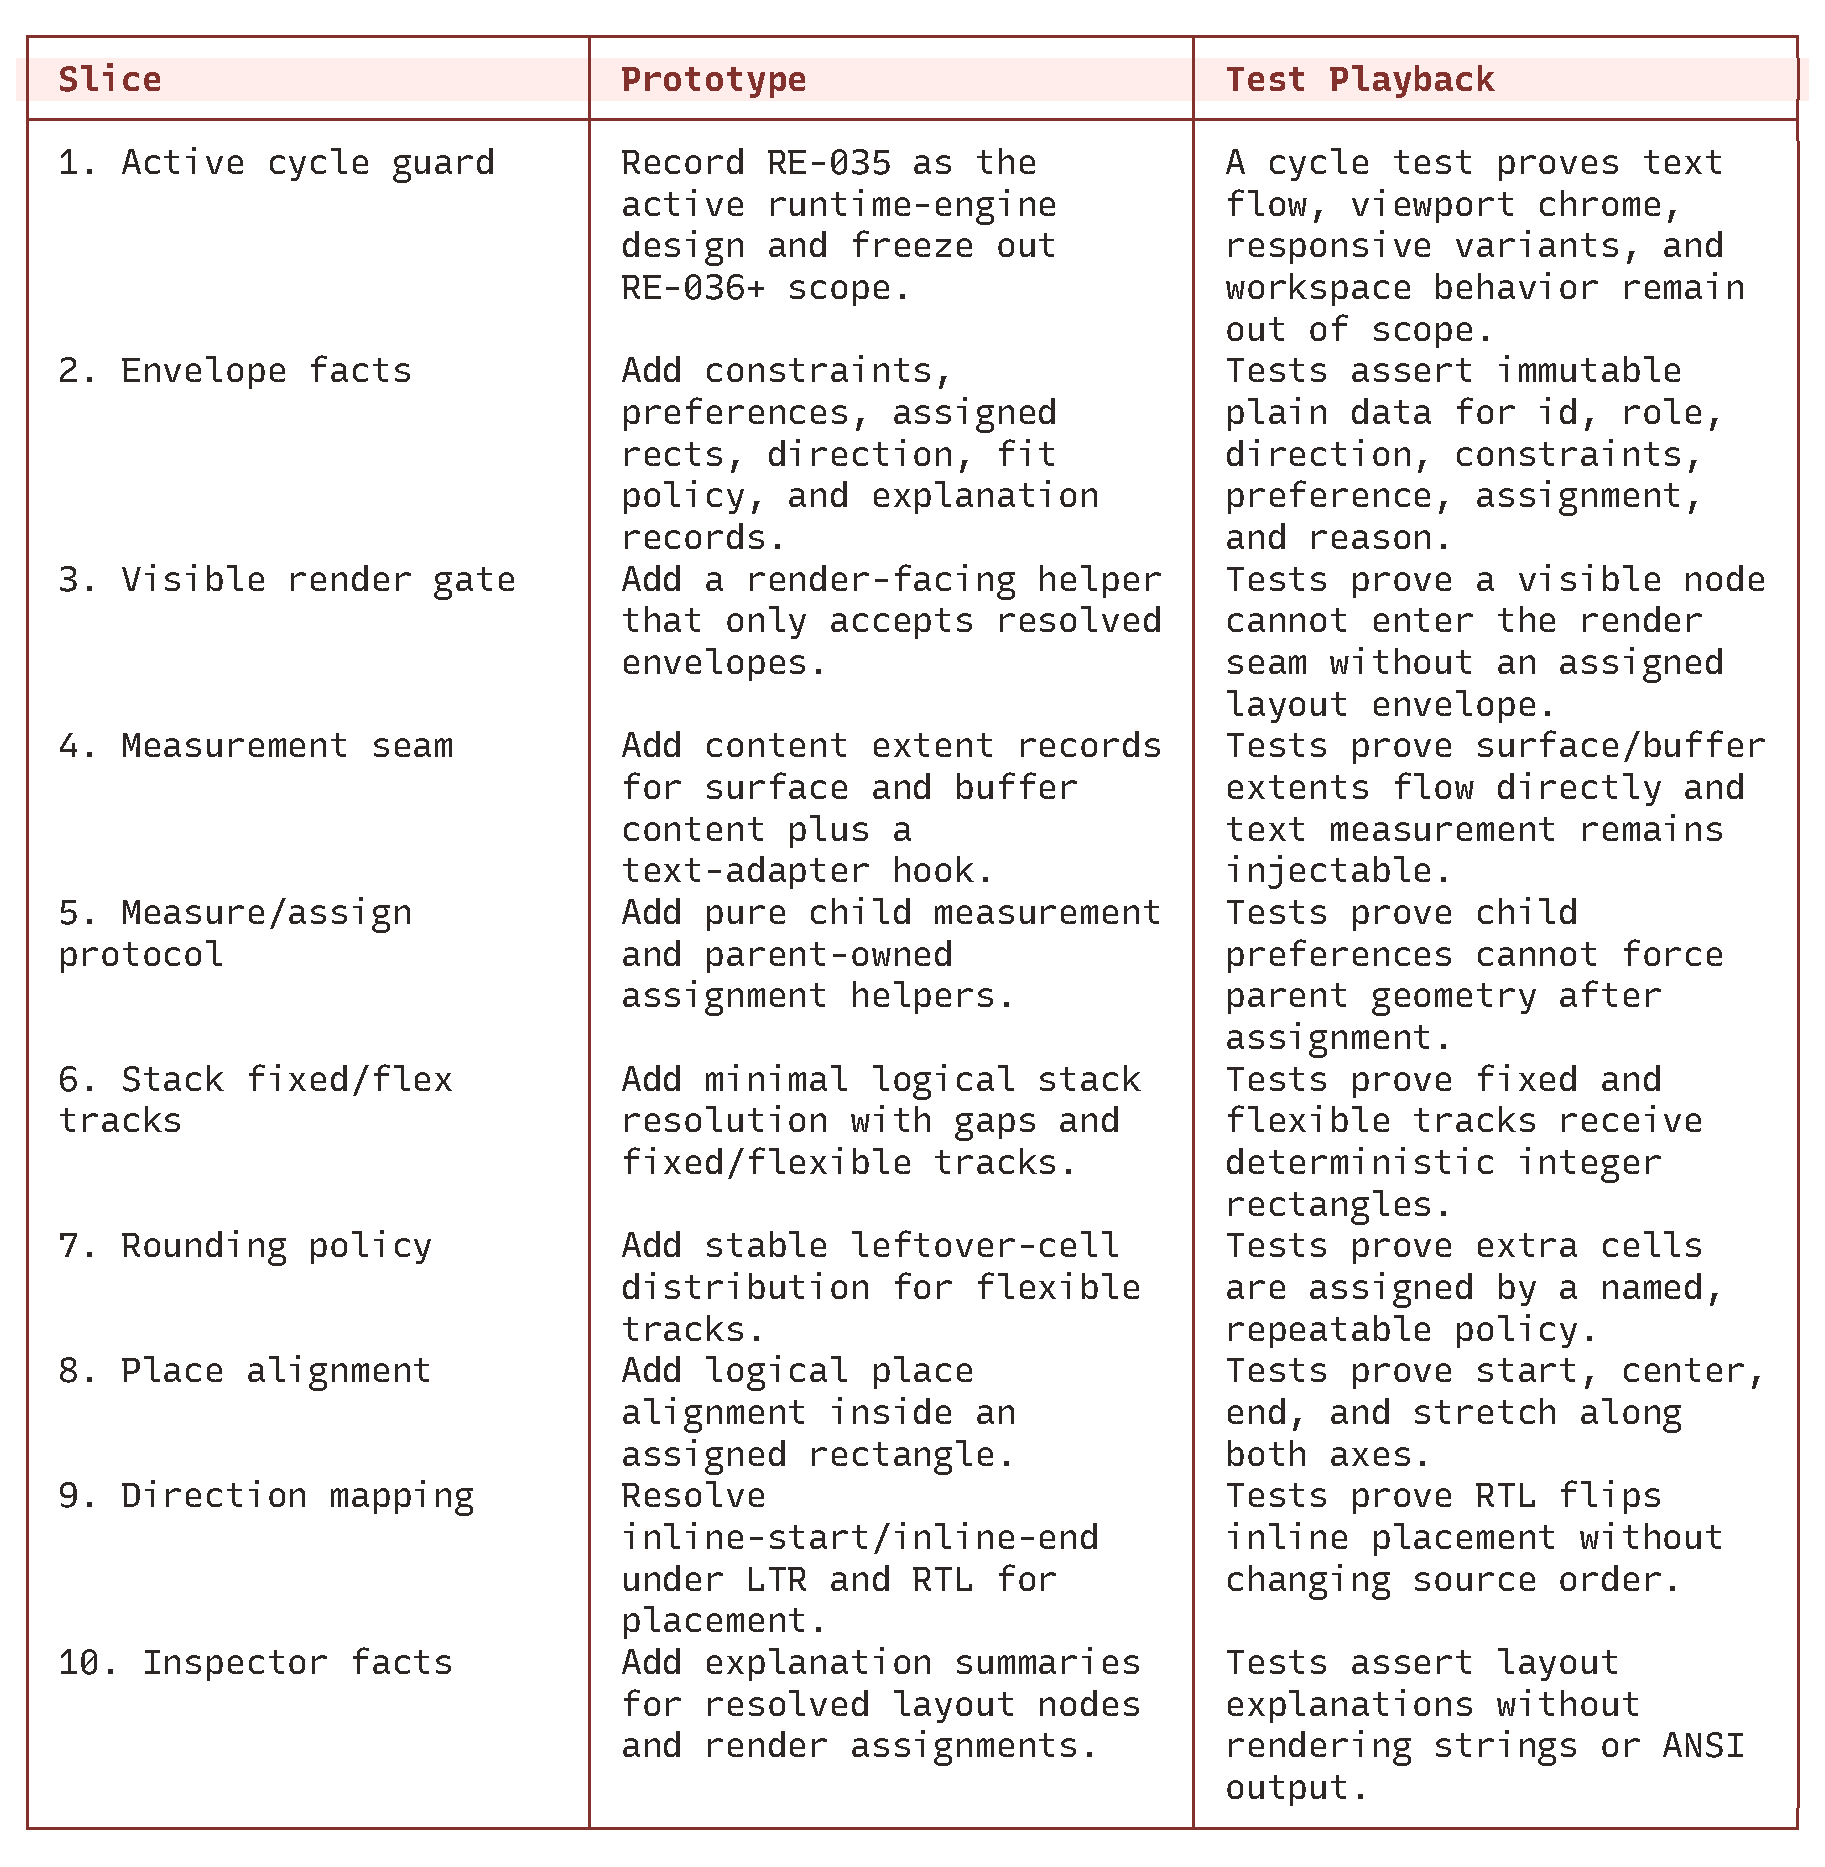
\includegraphics[width=\linewidth]{figures/tables/table-042-g1-1.pdf}
\par\smallskip{\scriptsize\color{BookMuted}Rows 1–10. Actual Bijou table component.}
\end{center}


\subsection{Playback Cadence}\label{record-163-playback-cadence}

\begin{itemize}
\tightlist
\item
  RED: write the slice test first, tied to the playback question above.
\item
  GREEN: add only the pure runtime code needed for that slice.
\item
  LEARN: update this design doc's Drift Check, Playback, and Retrospective when a slice changes the boundary or leaves follow-on debt.
\end{itemize}

\section{Tests To Write First}\label{record-163-tests-to-write-first}

\begin{itemize}
\tightlist
\item
  Cycle test proving RE-035 is the active runtime-engine design and that later text, viewport, chrome, responsive, and workspace work remains out of scope.
\item
  Package-local tests proving visible nodes require a layout envelope before rendering.
\item
  Package-local tests proving child preferences cannot force parent geometry.
\item
  Package-local tests proving stack assigns fixed and flexible tracks deterministically.
\item
  Package-local tests proving leftover cells are rounded by a stable policy.
\item
  Package-local tests proving \texttt{p\allowbreak{}l\allowbreak{}a\allowbreak{}c\allowbreak{}e} aligns children at logical start, center, end, and stretch.
\item
  Package-local tests proving RTL flips inline-start and inline-end placement.
\item
  Package-local tests proving layout explanation facts include node id, role, constraints, preferences, assigned rect, and reason.
\item
  Package-local tests proving a renderer receives the assigned rect from layout resolution.
\end{itemize}

\section{Acceptance Criteria}\label{record-163-acceptance-criteria}

\begin{itemize}
\tightlist
\item
  RED tests fail before implementation and pass after.
\item
  Visible UI nodes cannot enter the render-facing seam without a layout envelope.
\item
  Parent assignment is authoritative and deterministic.
\item
  Stack and place prove the minimum useful layout contract without full flexbox, scrollbars, or workspace behavior.
\item
  Surface and buffer content can report cell extents directly.
\item
  Text measurement remains an adapter seam, not the canonical layout model.
\item
  Layout explanations can be asserted without rendering a string.
\end{itemize}

\section{Risks / Unknowns}\label{record-163-risks-unknowns}

\begin{itemize}
\tightlist
\item
  The first contract may be too small for later viewport or workspace needs, so the types should stay extensible without accepting solver complexity.
\item
  Text measurement is the next hard problem, but it should not drag RE-035 into grapheme, bidi, and cursor-map work.
\item
  Existing string-returning component APIs may need compatibility wrappers while the retained layout path matures.
\item
  Mermaid diagrams in editor tooling can drift, so diagrams should stay conceptual and not become implementation specs.
\end{itemize}

\section{Future Sequence}\label{record-163-future-sequence}

RE-035 deliberately ships the floor, not the full system.

Follow-on cycles should stay layered:

\begin{itemize}
\tightlist
\item
  RE-036 Text Measurement And Inline Flow
\item
  RE-037 Overflow, Viewports, Scroll Anchoring, And Scrollbars
\item
  RE-038 Box Model, Chrome Regions, Hit Testing, And Focus Maps
\item
  RE-039 Responsive Variants, Compression, And Constraint Fallbacks
\item
  RE-040 Mode Lowering And Accessible Layout Semantics
\item
  WS-001 Workspace Tree: Panels, Tabsets, Docks, Drawers
\item
  WS-002 Workspace Interaction: Resize, Drag/Drop, Persistence
\end{itemize}

Workspace features compile into layout. Interaction emits commands. Rendering paints resolved rectangles. None of those layers should mutate layout geometry behind the layout engine's back.

\section{Drift Check}\label{record-163-drift-check}

Started on 2026-06-02 as a pure \texttt{@\allowbreak{}f\allowbreak{}l\allowbreak{}y\allowbreak{}i\allowbreak{}n\allowbreak{}g\allowbreak{}r\allowbreak{}o\allowbreak{}b\allowbreak{}o\allowbreak{}t\allowbreak{}s\allowbreak{}/\allowbreak{}b\allowbreak{}i\allowbreak{}j\allowbreak{}o\allowbreak{}u} core layout slice.

The first ten slices intentionally landed in \texttt{p\allowbreak{}a\allowbreak{}c\allowbreak{}k\allowbreak{}a\allowbreak{}g\allowbreak{}e\allowbreak{}s\allowbreak{}/\allowbreak{}b\allowbreak{}i\allowbreak{}j\allowbreak{}o\allowbreak{}u\allowbreak{}/\allowbreak{}s\allowbreak{}r\allowbreak{}c\allowbreak{}/\allowbreak{}c\allowbreak{}o\allowbreak{}r\allowbreak{}e\allowbreak{}/\allowbreak{}l\allowbreak{}a\allowbreak{}y\allowbreak{}o\allowbreak{}u\allowbreak{}t\allowbreak{}/} instead of \texttt{b\allowbreak{}i\allowbreak{}j\allowbreak{}o\allowbreak{}u\allowbreak{}-\allowbreak{}t\allowbreak{}u\allowbreak{}i}, DOGFOOD, or shell renderers. That keeps the contract mode-neutral and lets tests assert layout truth before any renderer paints.

Confirmed scope boundaries:

\begin{itemize}
\tightlist
\item
  stack and place are proof containers, not a full flexbox or workspace model
\item
  text content uses an injected measurement adapter, not JavaScript string length
\item
  render-facing code receives assigned rectangles through a seam, but existing components are not migrated in this slice
\item
  layout explanation facts are plain data and do not require ANSI output
\end{itemize}

\section{Playback}\label{record-163-playback}

RED:

\begin{itemize}
\tightlist
\item
  Added \texttt{p\allowbreak{}a\allowbreak{}c\allowbreak{}k\allowbreak{}a\allowbreak{}g\allowbreak{}e\allowbreak{}s\allowbreak{}/\allowbreak{}b\allowbreak{}i\allowbreak{}j\allowbreak{}o\allowbreak{}u\allowbreak{}/\allowbreak{}s\allowbreak{}r\allowbreak{}c\allowbreak{}/\allowbreak{}c\allowbreak{}o\allowbreak{}r\allowbreak{}e\allowbreak{}/\allowbreak{}l\allowbreak{}a\allowbreak{}y\allowbreak{}o\allowbreak{}u\allowbreak{}t\allowbreak{}/\allowbreak{}e\allowbreak{}n\allowbreak{}v\allowbreak{}e\allowbreak{}l\allowbreak{}o\allowbreak{}p\allowbreak{}e\allowbreak{}.\allowbreak{}t\allowbreak{}e\allowbreak{}s\allowbreak{}t\allowbreak{}.\allowbreak{}t\allowbreak{}s} before the module existed. The focused test failed because \texttt{.\allowbreak{}/\allowbreak{}e\allowbreak{}n\allowbreak{}v\allowbreak{}e\allowbreak{}l\allowbreak{}o\allowbreak{}p\allowbreak{}e\allowbreak{}.\allowbreak{}j\allowbreak{}s} was missing.
\end{itemize}

GREEN:

\begin{itemize}
\tightlist
\item
  Added immutable layout constraints, preferences, assigned rectangles, directions, fit policy, and resolved-envelope facts.
\item
  Added a render-facing seam that rejects unresolved visible nodes and passes parent-assigned rectangles to the renderer callback.
\item
  Added surface and buffer cell extent helpers plus an injected text measurement seam.
\item
  Added parent-owned child assignment, minimal stack fixed/flex layout, source-order largest-remainder rounding, place alignment, RTL inline start/end mapping, and inspectable explanation facts.
\item
  Exported the RE-035 primitives from \texttt{@\allowbreak{}f\allowbreak{}l\allowbreak{}y\allowbreak{}i\allowbreak{}n\allowbreak{}g\allowbreak{}r\allowbreak{}o\allowbreak{}b\allowbreak{}o\allowbreak{}t\allowbreak{}s\allowbreak{}/\allowbreak{}b\allowbreak{}i\allowbreak{}j\allowbreak{}o\allowbreak{}u}.
\end{itemize}

\section{Retrospective}\label{record-163-retrospective}

The first ten slices establish the boring floor: visible layout facts can now exist and be tested before rendering. The main restraint was keeping RE-035 from turning into RE-036 through RE-040. The current module deliberately does not solve text flow, overflow, hit testing, responsive fallbacks, accessible layout lowering, or workspace behavior.

Follow-on adoption should be separate and test-led: migrate one render-facing surface family at a time to consume assigned rectangles, then introduce text measurement, viewport overflow, and hit-test facts as their own cycles.

